%% This is an example first chapter.  You should put chapter/appendix that you
%% write into a separate file, and add a line \include{yourfilename} to
%% main.tex, where `yourfilename.tex' is the name of the chapter/appendix file.
%% You can process specific files by typing their names in at the 
%% \files=
%% prompt when you run the file main.tex through LaTeX.
\chapter{Introduction}
\label{chap:intro}

In past few years, the development of \textit{Robotics} has surpassed people's expectation. The word \textit{Robotics} has been first appeared in science fiction "Liar!" by Issac Asimov~\cite{wiki:Robotics}, it referred to science and technology of robots. By definition, \textit{Robotics} is a research branch that related to design, control and application of robots, as well as processing feedback from robots. 

Modern robots have been classified into several categories(\eg, Mobile robot, industrial robot, service robot, education robot \etc) with their usages. Among those categories, full-autonomous or semi-autonomous mobile robots attracts more and more researches. Such robots have abilities to move around in their moving space, with or without humans' control. The aim of research in mobile robots is to help us accomplish various hard tasks, whether domestically, commercially or militarily. These tasks, such as assisting disabled people, defusing bombs, or repair equipment in dangerous place is either risky or high expense for human beings.    

For mobile robot, finding physical location of itself in unknown environment is normally crucial, such an ability(\eg, \textit{Robot Navigation}) allows mobile robots avoid risky obstacles and finally arrive the goal position. Roughly speaking, \textit{Robot Navigation} is a computing system which processes the information from external sources(\eg, sensors) and apply an algorithm to navigate robot, and sometimes build a map of environment. In \textit{Robot Navigation}, robots sense environmental information by their sensors. These sensors, either locally (\eg, camera, inertial measurement unit (IMU)), or globally (\eg, Global Positioning System) detect events or changes in environment, and transfer their data to robots. Generally, sensors equipped in mobile robot (Local Sensor) are designed light,
small, and inexpensive considering convenient movement and low expense. Camera and IMU sensor are considered most common local sensor in small mobile robot system.

A camera is a optical instrument for capturing images. Modern camera has several advantages for \textit{Robot Navigation}. First, the core of camera chip set is cheap and easily installed in any mobile robot system; Second, camera often brings very rich information as it simulates the functioning of human eye. By recognizing key-points ~\cite{shi1994good, lowe1999object, rosten2010faster} in certain images, system observes the \textit{landmarks} in environment, and those \textit{landmarks} will localize robots by \textit{Triangulation} ~\cite{davison2003real, klein2007parallel, eade2007monocular}.

A IMU sensor (Figure~\ref{fig:fig1-1}) often combines \textit{gyroscope} and \textit{accelerometer}, sometimes \textit{magnetometer}, to measure specific force, angular rate and magnetic field regarding to its local frame. IMU is one of main component in \textit{Inertial Navigation System}, which firstly used in air plane, spacecraft, guided missiles, and now also in mobile robot ~\cite{batalin2004mobile, lee2009position, mourikis2007multi, forster2015imu}. IMU sensor utilize \textit{Dead Reckoning} to track device's position, such technology tries to integrate IMU data over time by assuming the movement model of devices fixed(\ie, acceleration and rotation rate is constant over small period of time). 

\begin{figure}
    \centering
    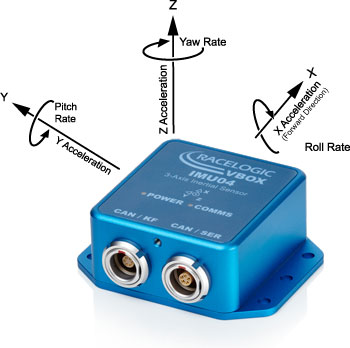
\includegraphics[width=0.5\textwidth]{CONTENT/Figure/Figure1-1_IMU_Sensor.jpg}
    \caption{IMU sensor with gyroscope and accelerometer measures rotational rate and acceleration of X, Y, Z axis regarding its local frame. Note that IMU sensor normally has bias and irreducible noises, it is necessary to apply a calibration like cameras. The frequency of IMU output is normally larger than 100 Hz. Source: \cite{Figure1-1_IMU_Sensor}}
    \label{fig:fig1-1}
\end{figure}


\section{Motivation and Contribution}
\label{sec:motiv_contrib}

The main motivation of this thesis is to improve the navigation accuracy by fusing camera data and IMU sensor data. 

Single sensor-based navigation system may not satisfy the requirements of high-quality localization by mobile robot. GPS-based navigation system has been used for outdoor devices for long time. However, such a system suffered from localizing in in-door environment, and also the accuracy of general GPS is not high, \ie, 3 to 5 meters error \cite{wiki:GPS}. For mobile robot, which may move from in-door to out-door, and requires high-accuracy navigation, GPS is mostly not used, or as baseline of navigation~\cite{hesch2014consistency}.   

Vision-based navigation system \cite{davison2003real, klein2007parallel}, or simultaneous localization and mapping (SLAM)~\cite{davison2007monoslam, engel2014lsd, mur2015orb} gives an acceptable navigation result. \cite{davison2003real} recognizes corner feature by single camera, and it uses a extended kalman filter framework to track the uncertainty and propagates the system state, however it can not handle large-scale scene. \cite{klein2007parallel} utilizes key-frame based bundle adjustment to update the map, improves both accuracy and efficiency, it still met some problem in large-scale scene, becasue vision-based method often is a trade-off between computational complexity and localization accuracy due to the rich information and low output frequency by camera. 

Single \textit{Inertial Navigation System} recognize its pose by \textit{Dead Reckoning}~\cite{mcnaughton1991dead, levi1996dead}. However, the problem of \textit{Dead Reckoning} error accumulation; Only few directions are observable~\cite{hesch2014consistency} by IMU during whole navigation process. When object corrupts movement assumption, a correction step by external data will be needed.

Fusing camera and IMU data has many advantages. On the one hand, it can decrease computational time by making good use of high-frequency IMU data; On the other hand, it can reduce the error accumulation of IMU integration by the correction of vision-based navigation result within several turn. Fuse the camera and IMU data for robot navigation is not novel. \cite{mourikis2007multi} applies multi-state kalman filter (MSCKF) on state update, decrease the computational complexity by only keeping few last information of keyframe. \cite{hesch2014consistency} analysis the consistency of MSCKF, correct the ways of IMU integration to obtain consistency of sytem, therefore increase the accuracy. \cite{forster2015imu} exploits a way to optimize manifold information, therefore solving data fusing problem in a non-linear optimization scheme. Unfortunately, codes and data of above methods are not accessible, that motivates to explore possible methods to increase accuracy of \textit{vision-inertial navigation system} both theoretically and experimentally.

The contributions of this thesis are as follows,
\begin{itemize}
\item {We exploit a highly flexible, realistic software to generate synthetic IMU sensor data and corresponding vision data, that is the main source to provide experimental data in this thesis.}
\item {We present error-state kalman filter system kinematic based on quaternion, explore the multiple ways to integrate IMU data due to different movement models.}
\item {We propose a novel method to update fusing result based on key-framed bundle adjustment.}
\item {We propose a real-time visual-inertial framework implemented in C\texttt{++}, which is stable, scalable, high-accuracy and low-latency.}
\end{itemize}

\section{Outline of the Thesis}
\label{sec:outline}

In Chapter \ref{chap:Overview} we first overview our visual-inertial odometry, including world representation, important notations, we also compare filter method and key-frame based method in SLAM problem, and in the end we explain our choice in this thesis.

Then we enter the Chapter \ref{chap:background}, which introduces \textit{Quaternion Algebra}. In this chapter, we introduces the basic operations on quaternion, the relationship among quaternion, rotation matrix and rotation vector. In this chapter, we also explain how to integrate or derivative quaternion over time.

Chapter \ref{chap:sensor_fusing} is main part of this thesis. In Section \ref{sec:ESKF_IMU}, we study the Error-State Kalman Filter (ESKF), and apply it to IMU integration; Section \ref{sec:camera_comple_data} we summarize how to fuse camera into ESKF, and how to optimize it by key-frame based bundle adjustment. In Section 
\ref{sec:pipeline_summary}, we overview the pipeline of our visual-inertial odometry system.

We show our experiment results in Chapter \ref{chap:experiments}. First, the process of generating synthetic IMU and camera data is presented. Then we run several experiments to show our proposed visual-inertial odometry has higher accuracy than  single IMU integration, visual SLAM, as our system is still running in real-time.

In the end, we summarize and discuss our work and analysis the potential future work in Chapter \ref{chap:summary}.
